\section{Abstract}

\begin{frame}{Abstract}
    
    Noiseprint~\cite{cozzolino2018noiseprint} is a CNN-based method, born for tampering detection, able to extract a camera model fingerprint, resistant to scene content and enhancing model-related artifacts. In this presentation, we show the results of testing Noiseprint against a dataset~\cite{montibeller} of out-camera images edited with modern post-processing software.
    
    \begin{figure}
        \centering
        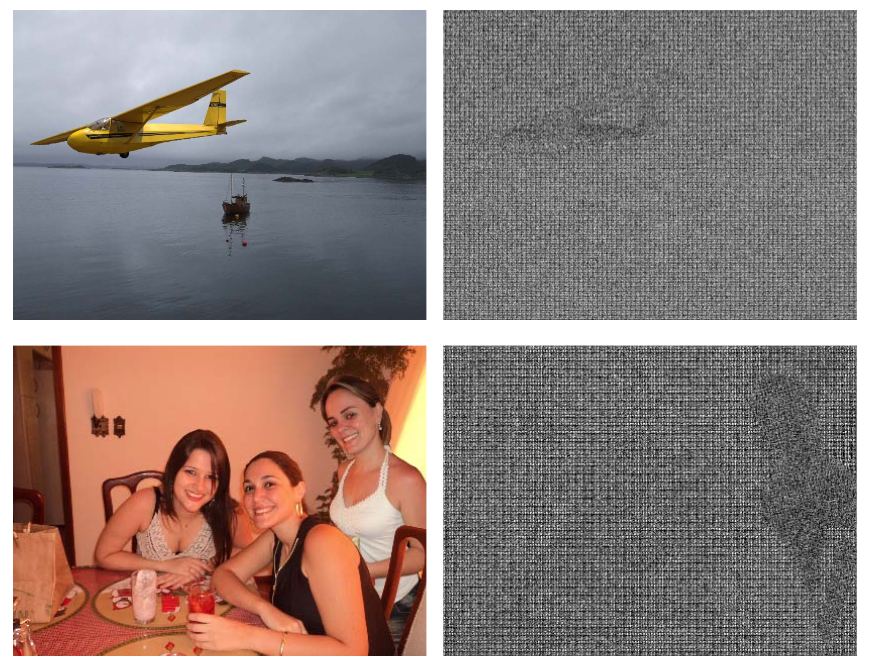
\includegraphics[width=0.44\textwidth]{../drawable/examples/example-noiseprint.png}
        \caption{Example of a Noiseprint extraction.}
    \end{figure}
\end{frame}

\section{Introduction}

\begin{frame}{Problem}

    Noiseprint~\cite{cozzolino2018noiseprint}'s original goal was to provide a tampering detection technique, but further studies outlined that it happened to provide acceptable results in the field of camera model identification.
    
    \medskip
    
    \begin{figure}
        \centering
        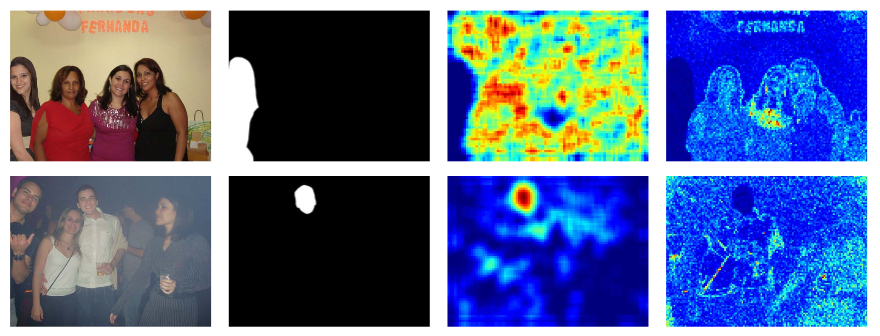
\includegraphics[width=0.6\textwidth]{../drawable/examples/example-tampering.png}
        \caption{Example of tampering detection with Noiseprint.}
    \end{figure}
    
    \medskip
    
    \onslide<2->{
        While being a relatively new paper (2018), Noiseprint has been trained on quite old and free-from-edits image database, the Dresden database~\cite{dresden}. 
    }
    
\end{frame}
\begin{frame}{Problem}
    
    This database features in-camera photographs from models released in the late 2000s, and none of them feature any kind of image manipulation.
    
    \medskip

    \onslide<2->{
        We aim to verify if the results on the Noiseprint paper are replicable on photos edited using image post-processing software.
    }
    
\end{frame}

\begin{frame}{Dresden database}

    The Dresden database used in this presentation is a narrowed down variant~\cite{dresden}.
    
    \begin{itemize}
        \item<2-> \textbf{9458} photos: \begin{itemize}
            \item<3-> \textbf{27} camera models
            \item<3-> between \textbf{80} and \textbf{1357} photos per model
            \item<4-> \textbf{73} different devices
            \item<4-> between \textbf{1} and \textbf{4} devices per model
        \end{itemize}
    \end{itemize}

    \begin{figure}
        \centering
        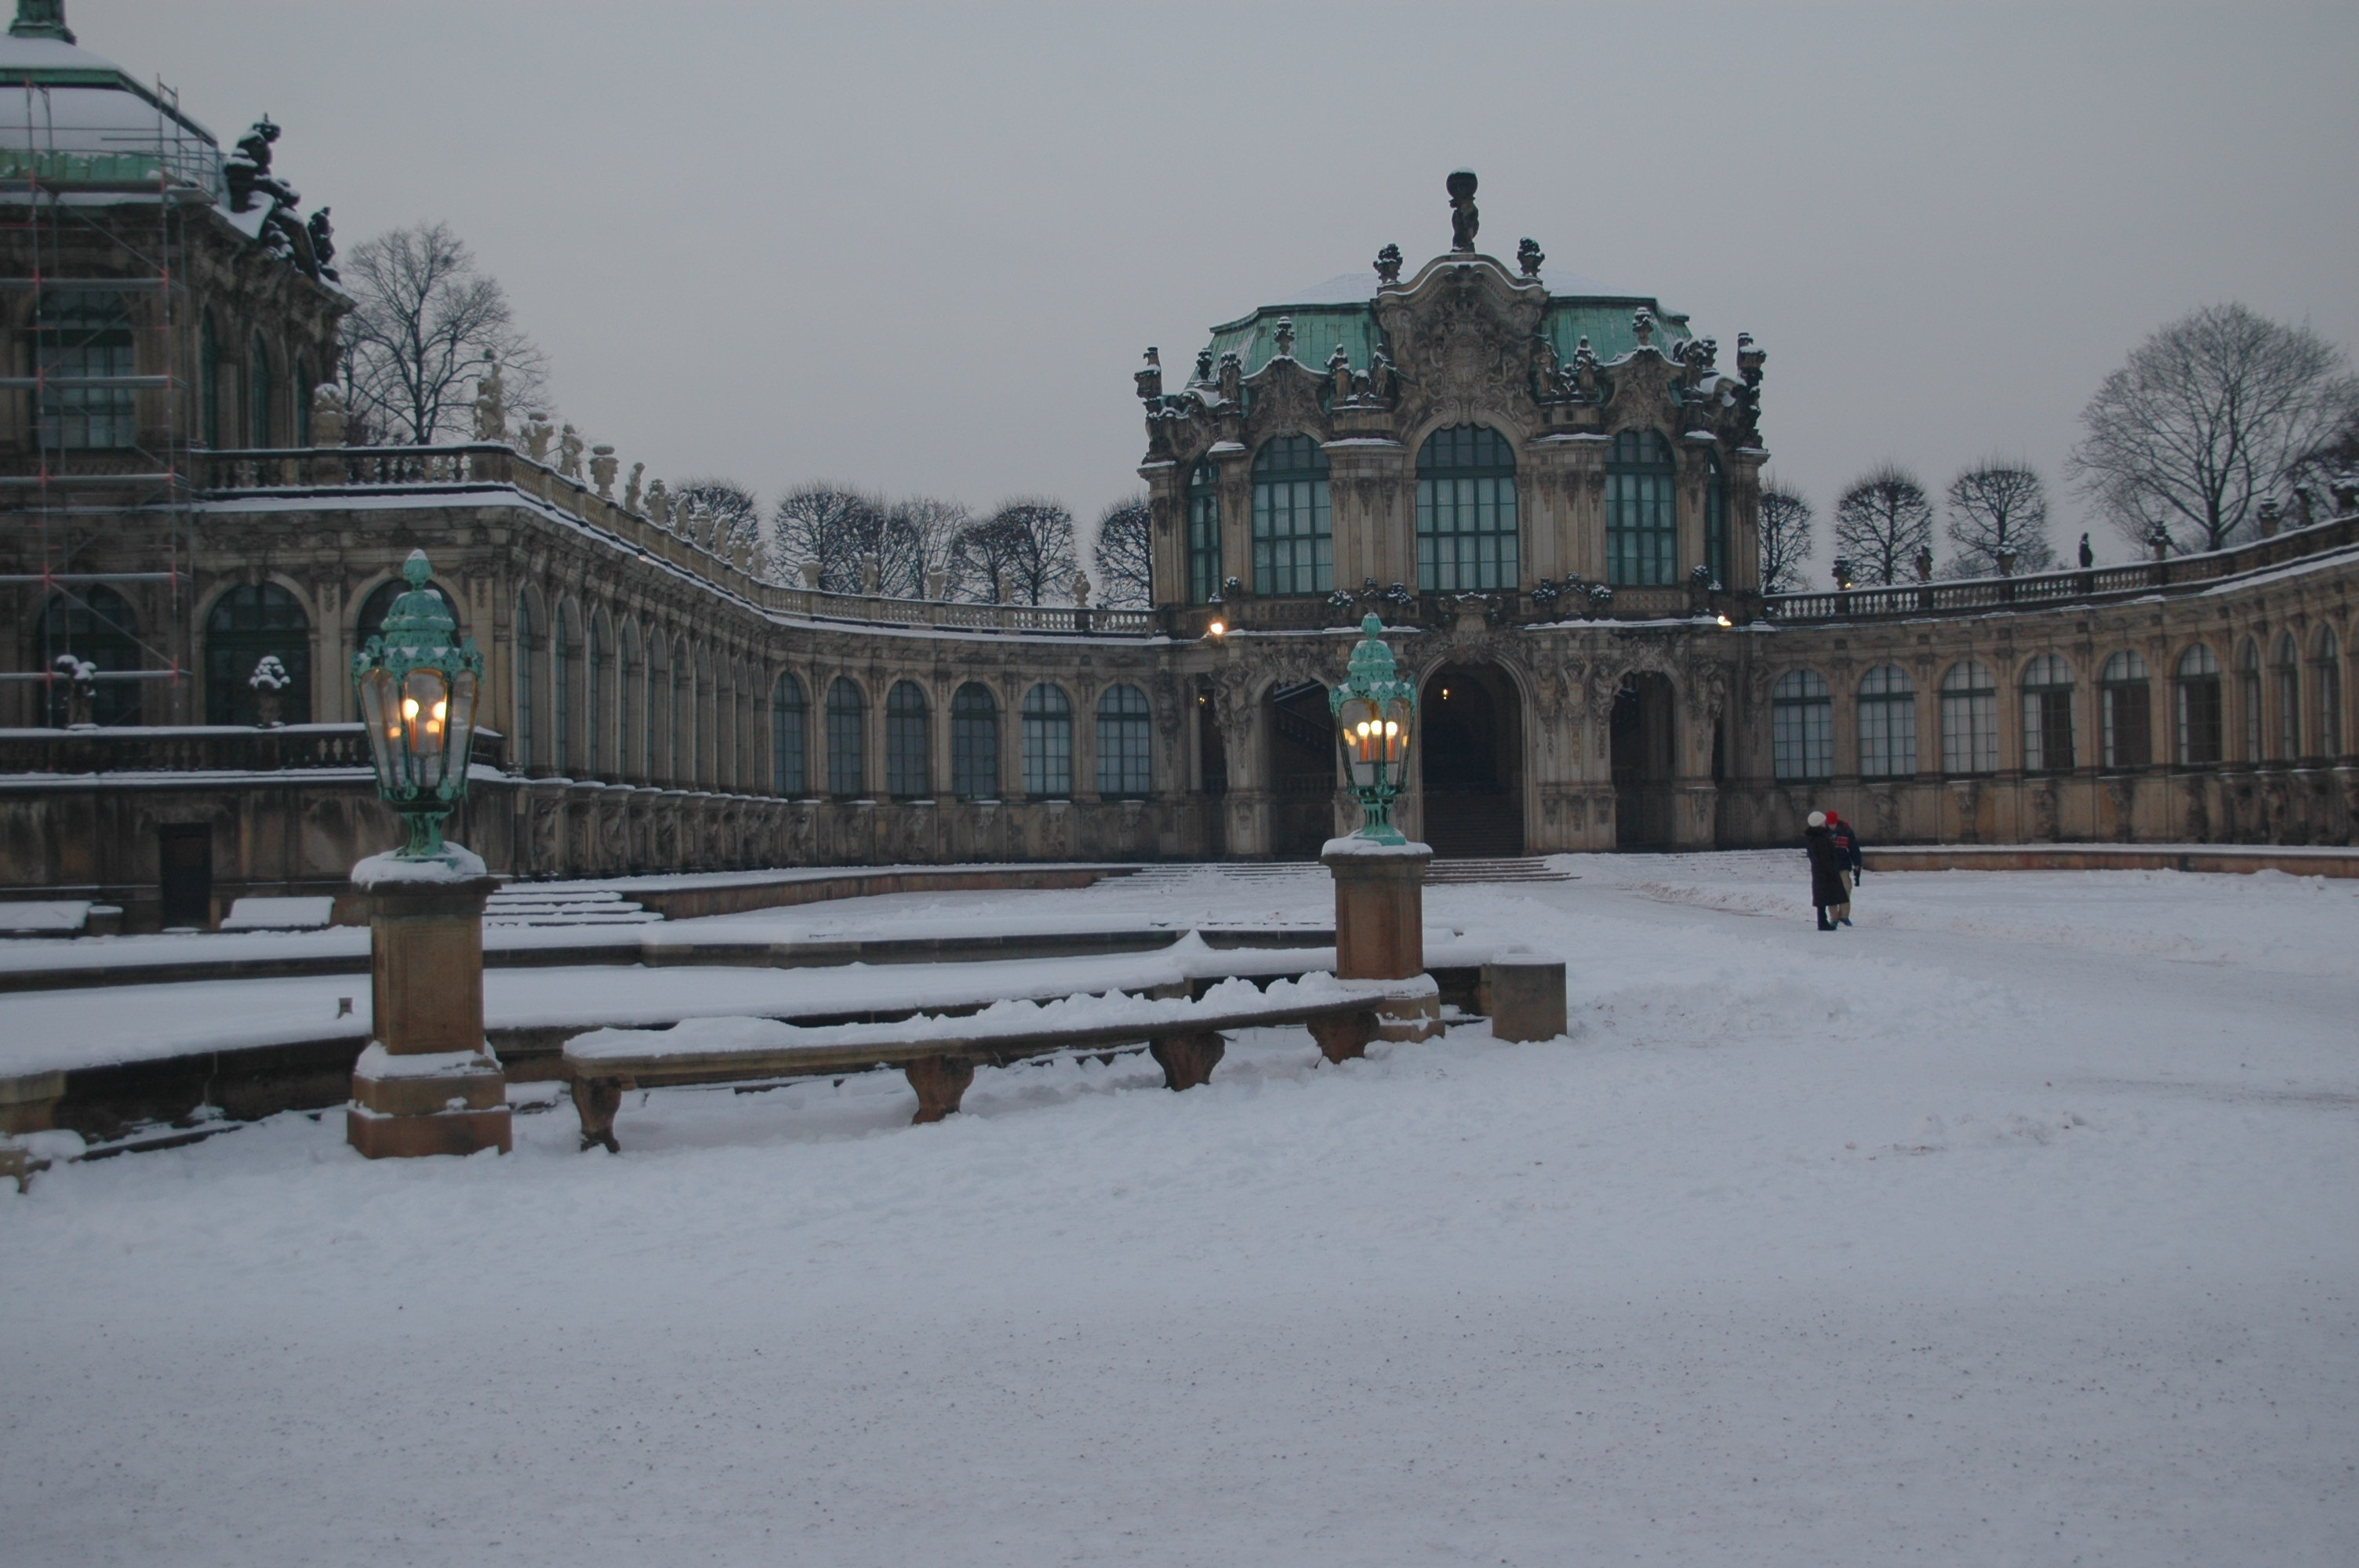
\includegraphics[width=0.6\textwidth]{../drawable/examples/example-dresden-D70_0_19451.JPG}
    \end{figure}
    
\end{frame}

\begin{frame}{Outcamera database}

    \begin{itemize}
        \item<1-> \textbf{821} photos shot by Andrea Montibeller~\cite{montibeller}: \begin{itemize}
            \item<2-> \textbf{20} clean images, for the fingerprint
            \item<3-> the others received radial correction with \textbf{Gimp}, \textbf{PTLens}, \textbf{Adobe Photoshop}, and \textbf{Adobe Lightroom}
            \item<4-> a fifth group contains photos corrected with a purposedly wrong camera profile
        \end{itemize}
    \end{itemize}
    
    \begin{figure}
        \centering
        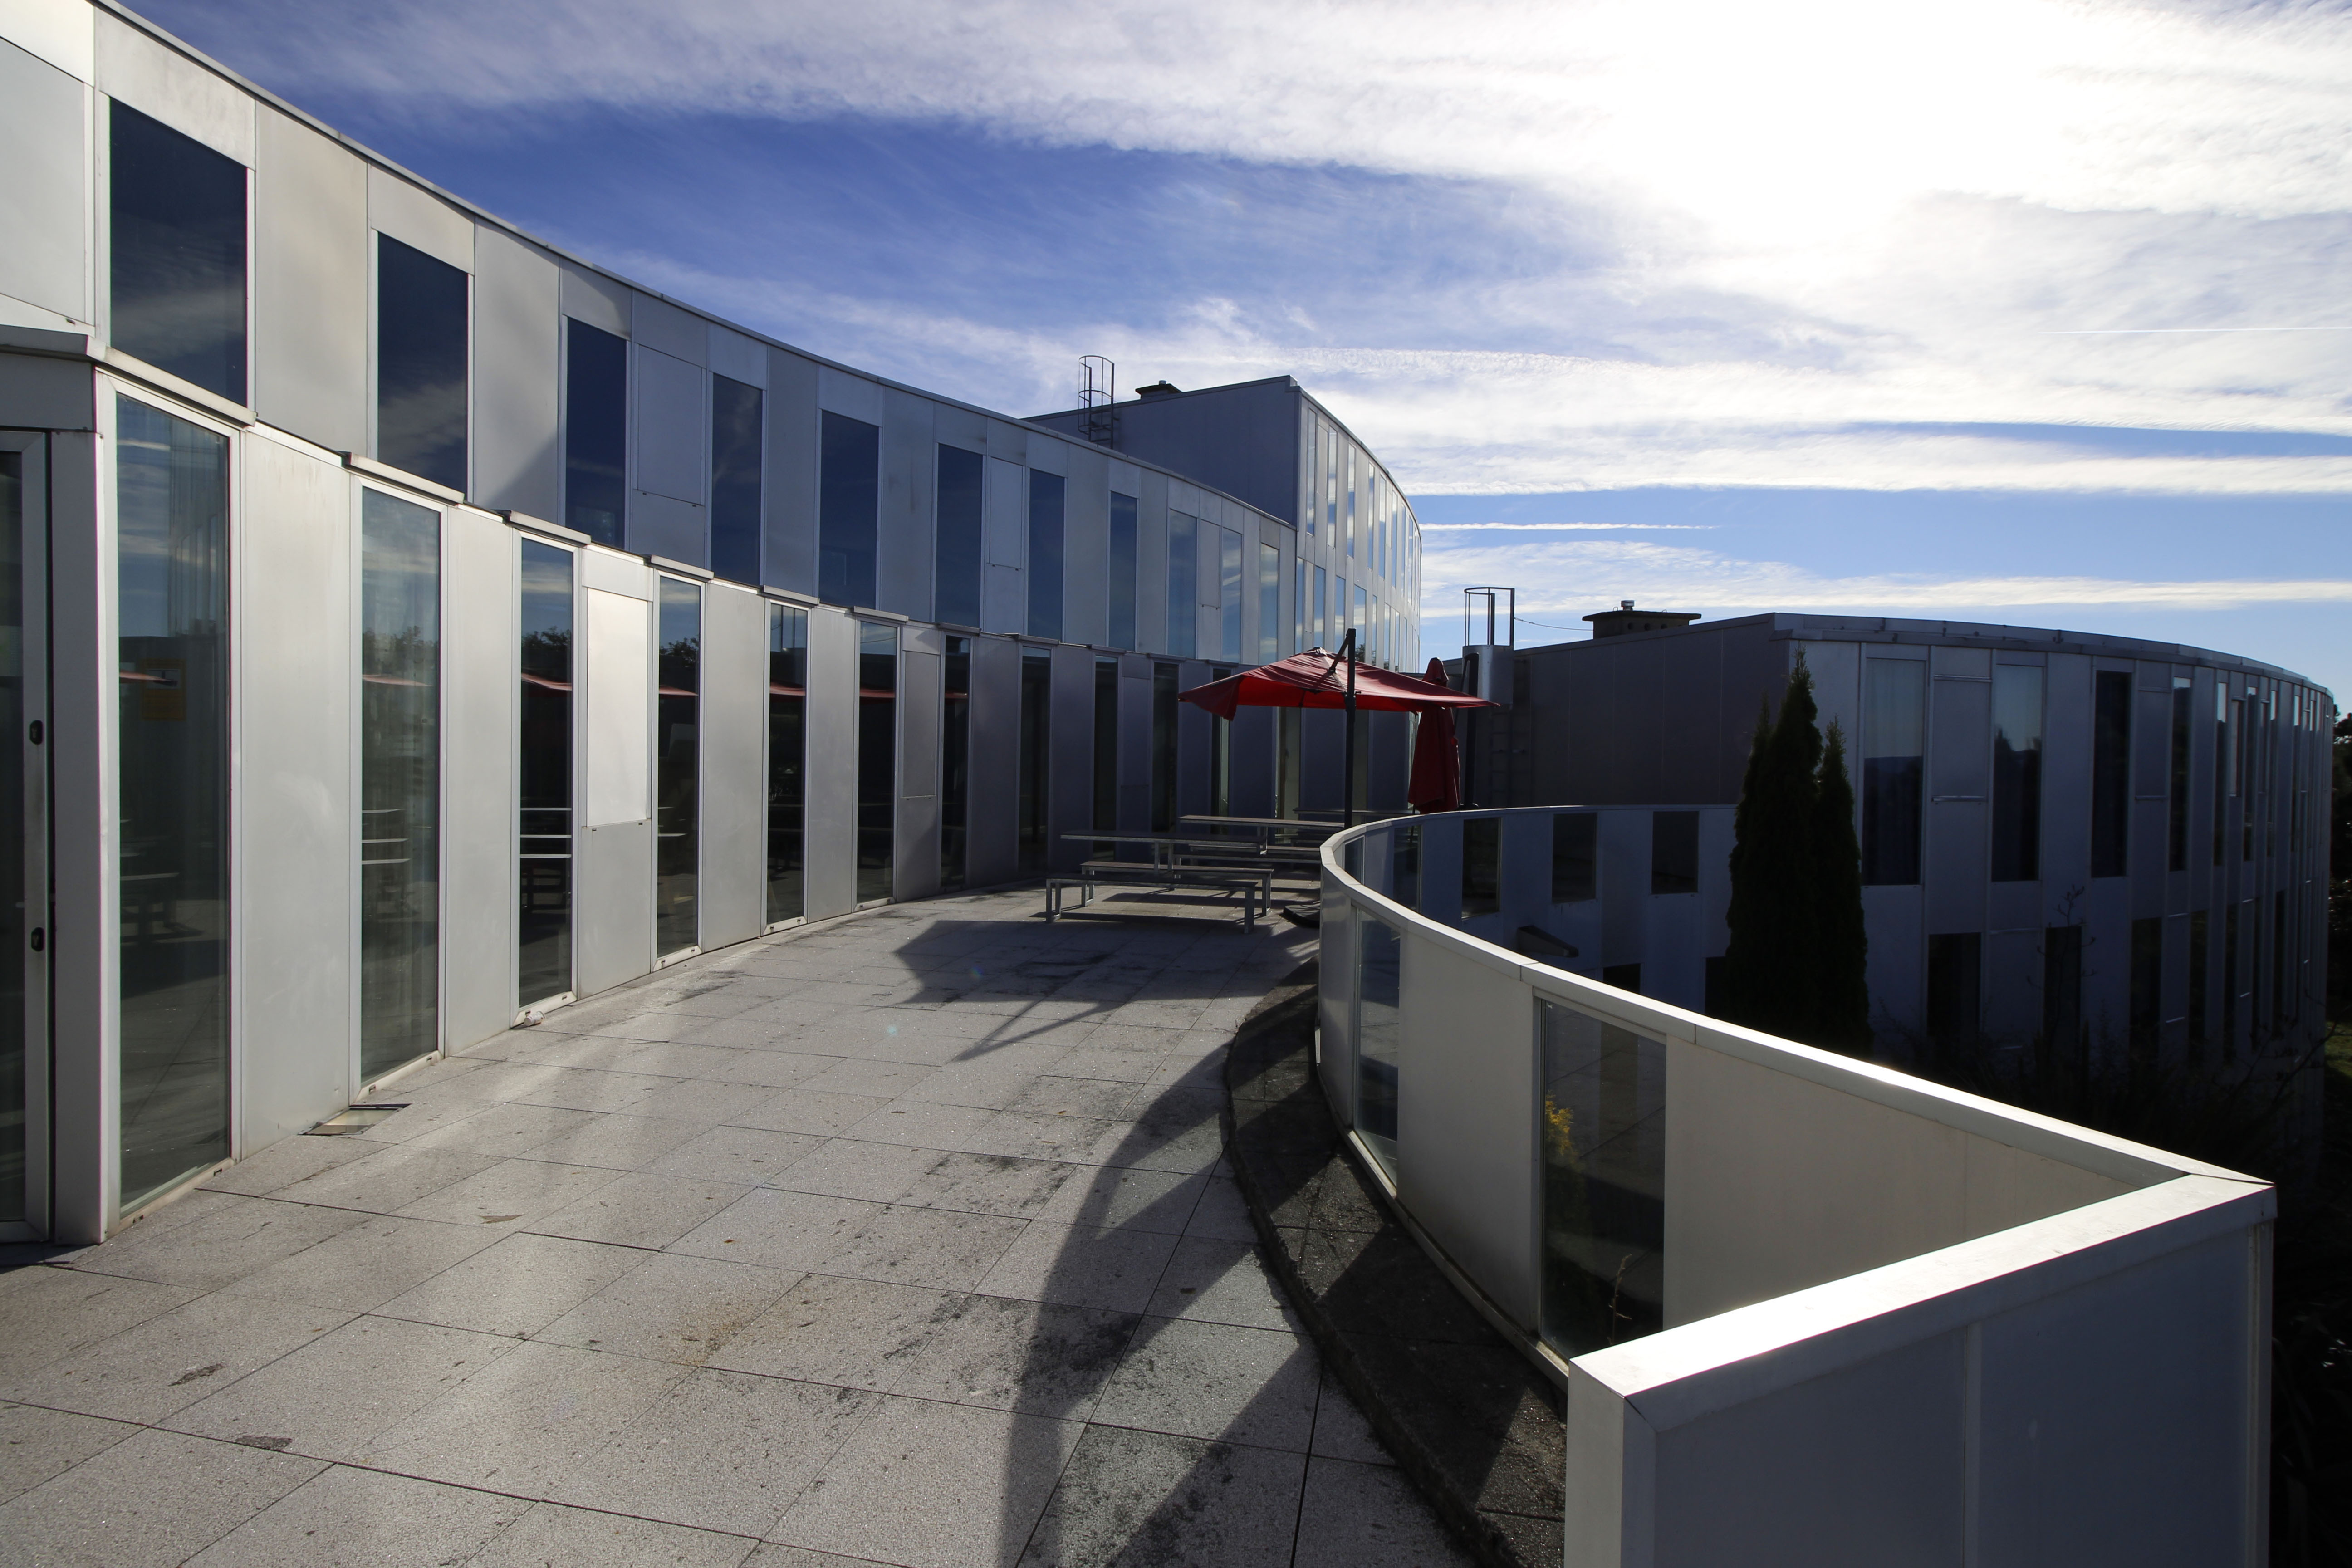
\includegraphics[width=0.66\textwidth]{../drawable/examples/example-outcamera-im24.jpg}
    \end{figure}
    
\end{frame}

\begin{frame}{Expected output}

    We want to obtain a handful of ROC curves that show us the performance of Noiseprint on both datasets.
    
    \medskip
    
    To obtain this, we will:
    
    \begin{itemize}
        \item<2-> filter the datasets to make them comparable;
        \item<3-> choose $N$ pictures for each camera model (27 + 1) to calculate a camera fingerprint;
        \item<4-> for each camera model (Dresden) / group (Outcamera) of the two datasets: \begin{itemize}
            \item choose $M$ pictures of the subset for the \texttt{H1} hypothesis;
            \item choose $M$ random pictures from other \textit{Dresden} pictures for \texttt{H0};
            \item calculate \textit{normalized cross-correlation} for each \texttt{H0/H1} picture and plot the results.
        \end{itemize}
    \end{itemize}
    
    % TODO mettere un disegnino?
    
\end{frame}

\section{Execution}

\subsection{Preparation}

\begin{frame}{Balancing the datasets}

\begin{figure}
    \centering
    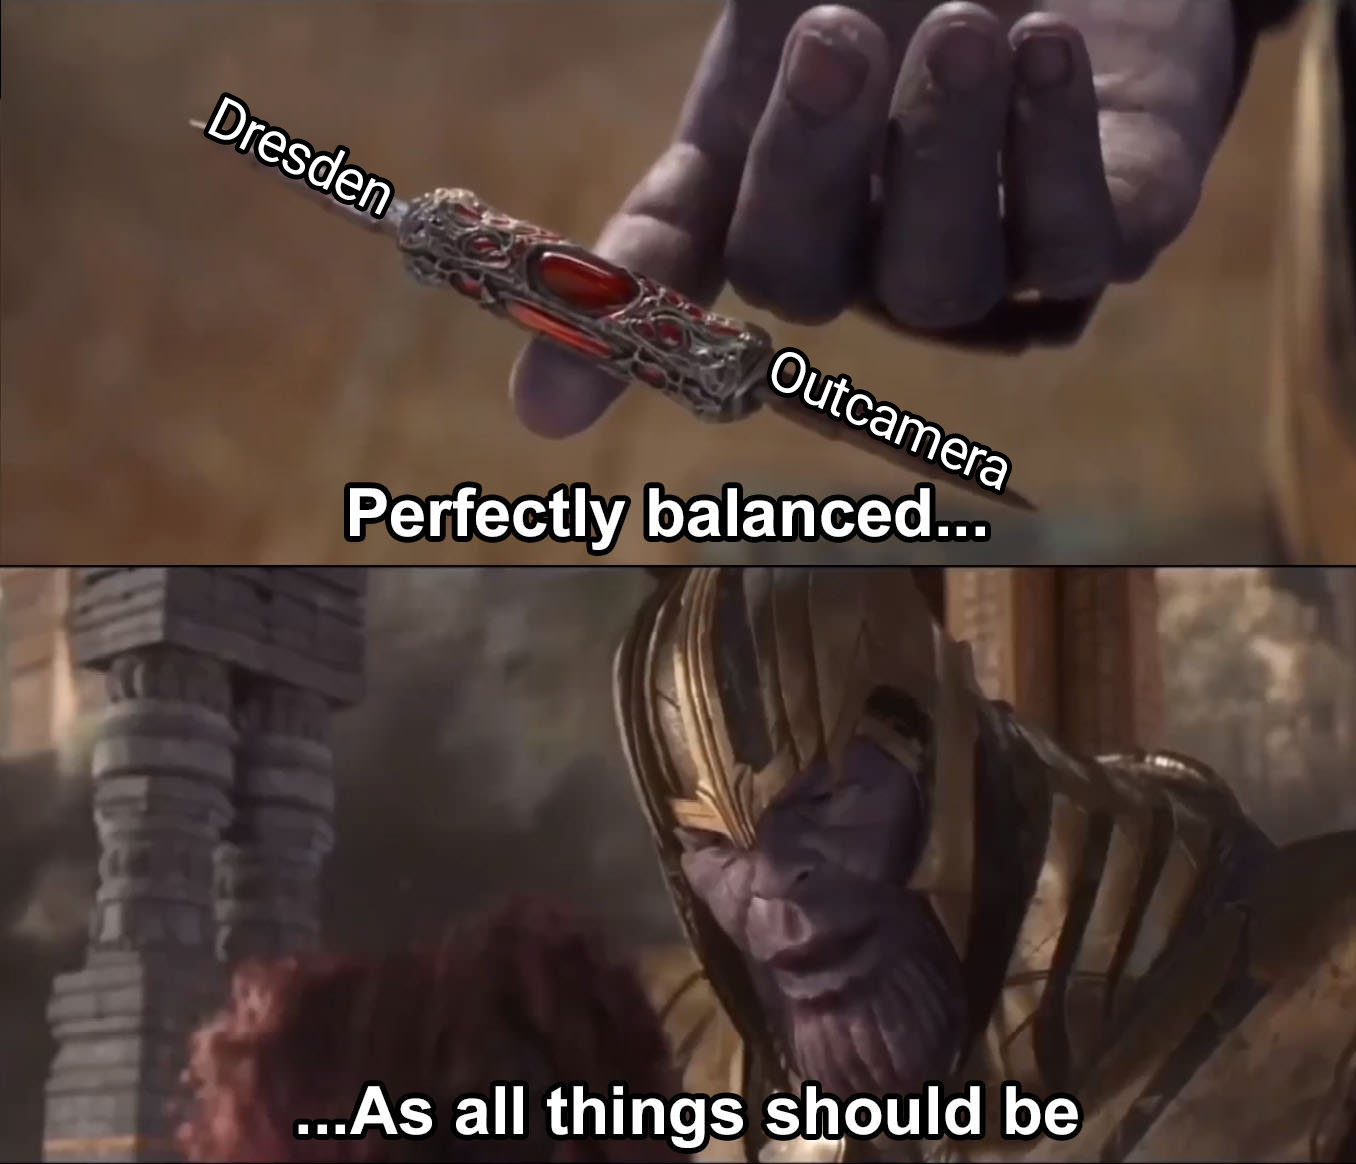
\includegraphics[height=0.78\textheight]{../drawable/meme.png}
\end{figure}
    
\end{frame}

\begin{frame}{Data selection (Outcamera)}

    The dataset - with only Canon 1200D images - has 
    
    \begin{itemize}
        \item \textbf{20} images for creating a camera fingerprint (as required) $\Rightarrow$ all fingerprints will require \textbf{20} images each. 
        \item \textbf{801} edited images \begin{itemize}
            \item divided into groups of roughly \textbf{160} pictures each
        \end{itemize}
    \end{itemize}
    
    \medskip 
    
    \onslide<2->{
        For each group (5 total):
        \begin{itemize}
            \item \textbf{160} \texttt{H1} pictures of the group itself
            \item \textbf{160} \texttt{H0} pictures chosen at random from the Dresden database
        \end{itemize}
    }
    
\end{frame}

\begin{frame}[fragile]{Data selection (Dresden)}

    Since our goal is to make an unbiased test, we will make this dataset uniform w.r.t. Outcamera and extract roughly \textbf{800} photos, obtaining a mini Dresden dataset.
    
    \medskip
    
    \onslide<2->{
        To further make it uniform over camera models, we extract 30 photos from each camera\footnote{ $30 \approx \frac{801}{27}$, where 801 is the amount of photos in the Outcamera dataset, and 27 is the number of cameras in the Dresden dataset}.
    }
    
    \medskip
    
    \onslide<3->{
        
        For each model:
        \begin{itemize}
            \item \textbf{30} \texttt{H1} pictures
            \item \textbf{30} \texttt{H0} pictures randomly chosen from other models
        \end{itemize}
    
    }

\end{frame}

\begin{frame}[fragile]{Data selection}
    
    \begin{figure}
        \centering
        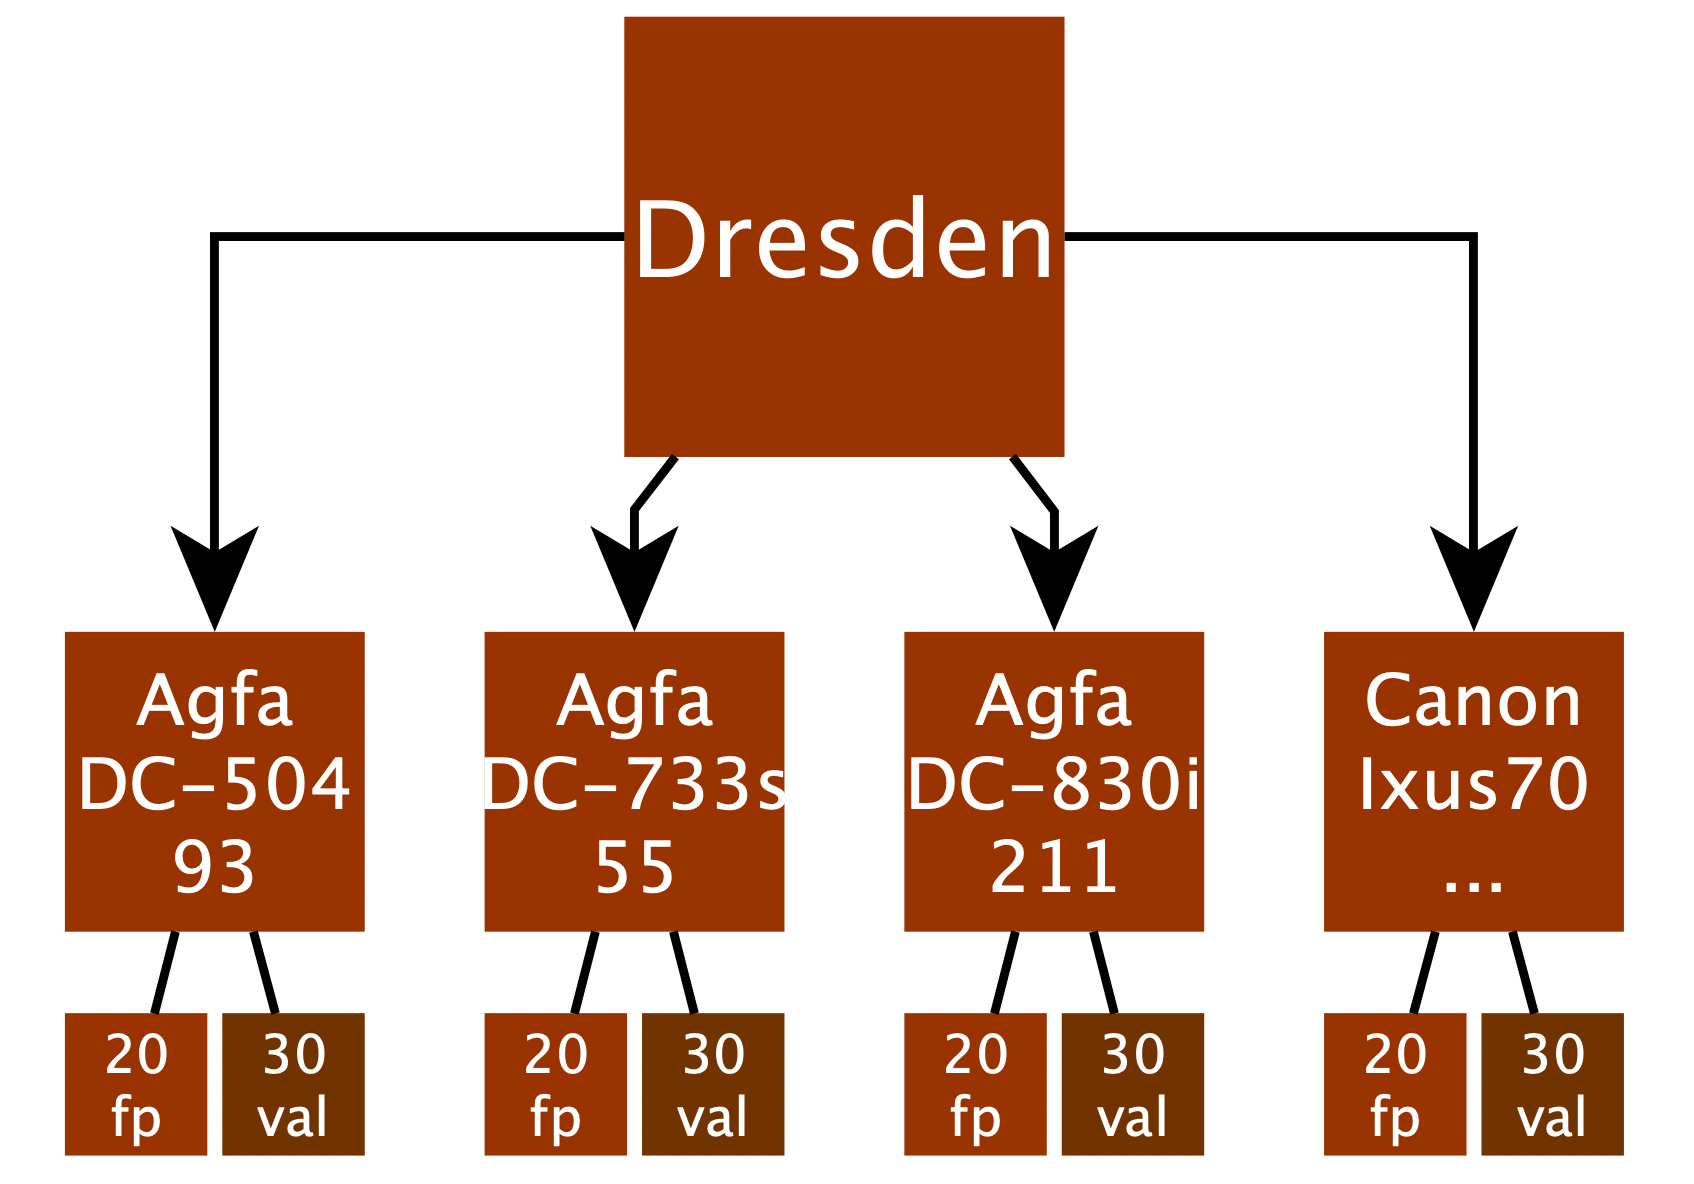
\includegraphics[width=0.8\textwidth]{../drawable/diagram.png}
    \end{figure}
    
\end{frame}

\subsection{Data extraction}

\begin{frame}[fragile]{Camera fingerprints}

    \begin{enumerate}
        \item verify that all chosen images from the same camera have same size
        \item use a parallel script for extracting each Noiseprint (for convenience, we extract \textbf{all} of them)
    \end{enumerate}
    
    \medskip
    
    \begin{lstlisting}
python3 noiseprint/main_extraction.py "$image"
    "$OUTDIR/${image//\.JPG/}.mat"
    \end{lstlisting}
    
    \medskip
    
    \onslide<2->{
        $\Rightarrow$ the fingerprint of each camera model is the average of its 20 image Noiseprints
    }
    
\end{frame}

\subsection{Validation}

\begin{frame}{Cross-correlating images}

    With the \texttt{.mat} files ready, for each fingerprint $FP$ another script: 
    
    \begin{itemize}
        \item<2-> selects the \texttt{H1} images available and randomly chooses $K$ images for the \texttt{H0} case\footnote{30 for Dresden, 160 for Outcamera};
        \item<3-> obtains a $1024 \times 1024$ central crop of each image;
        \item<4-> computes $ncc$ for each \texttt{H1} and \texttt{H0} image against $FP$;
        \item<5-> dumps the results to a JSON for later analysis.
    \end{itemize}
    
\end{frame}

%\begin{frame}{Final steps}
%    With the results readily available in JSON format, a final Python script computes a relevant visualization of data depending on the request (e.g. ROC curve, confusion matrix, table).
%\end{frame}

\section{Results}

\begin{frame}{ROC curves}
    \begin{figure}
        \centering
        \subfloat{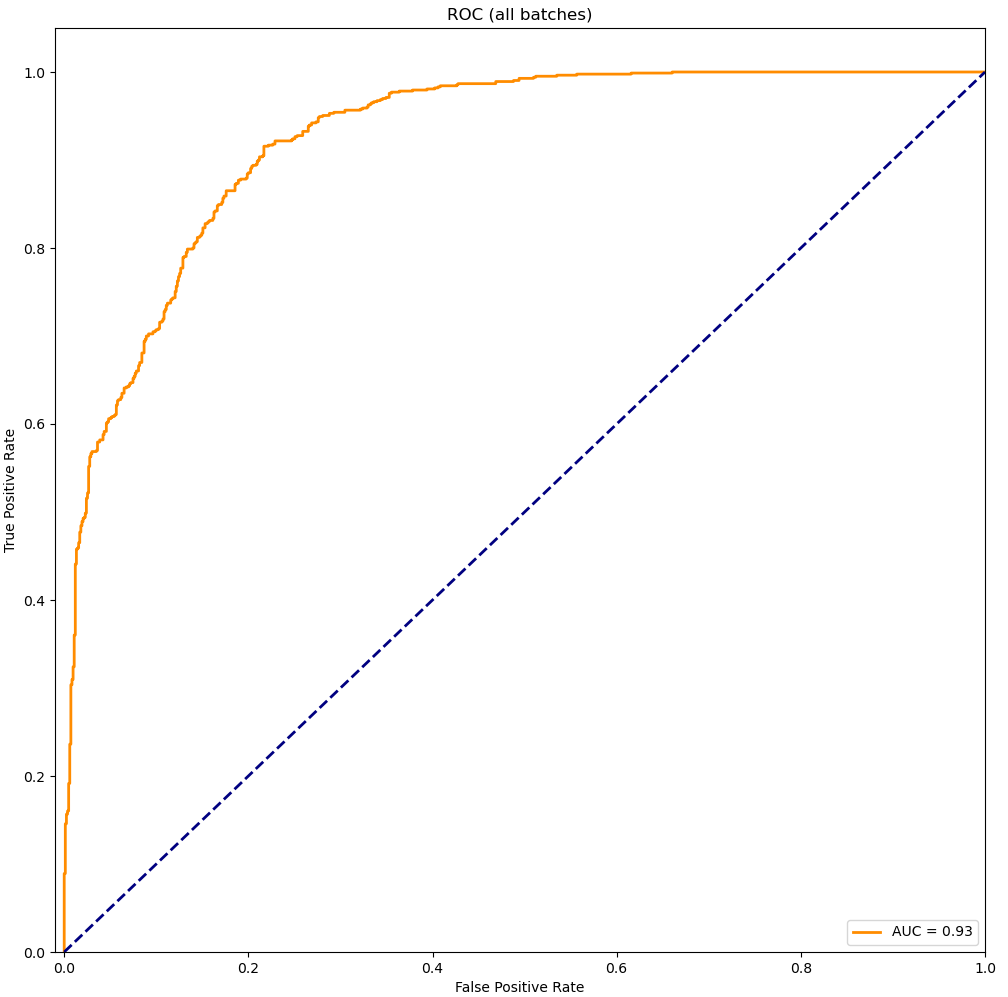
\includegraphics[width=.48\textwidth]{../drawable/results/roc-bulk__9252-all-dresden.png}} \quad
        \subfloat{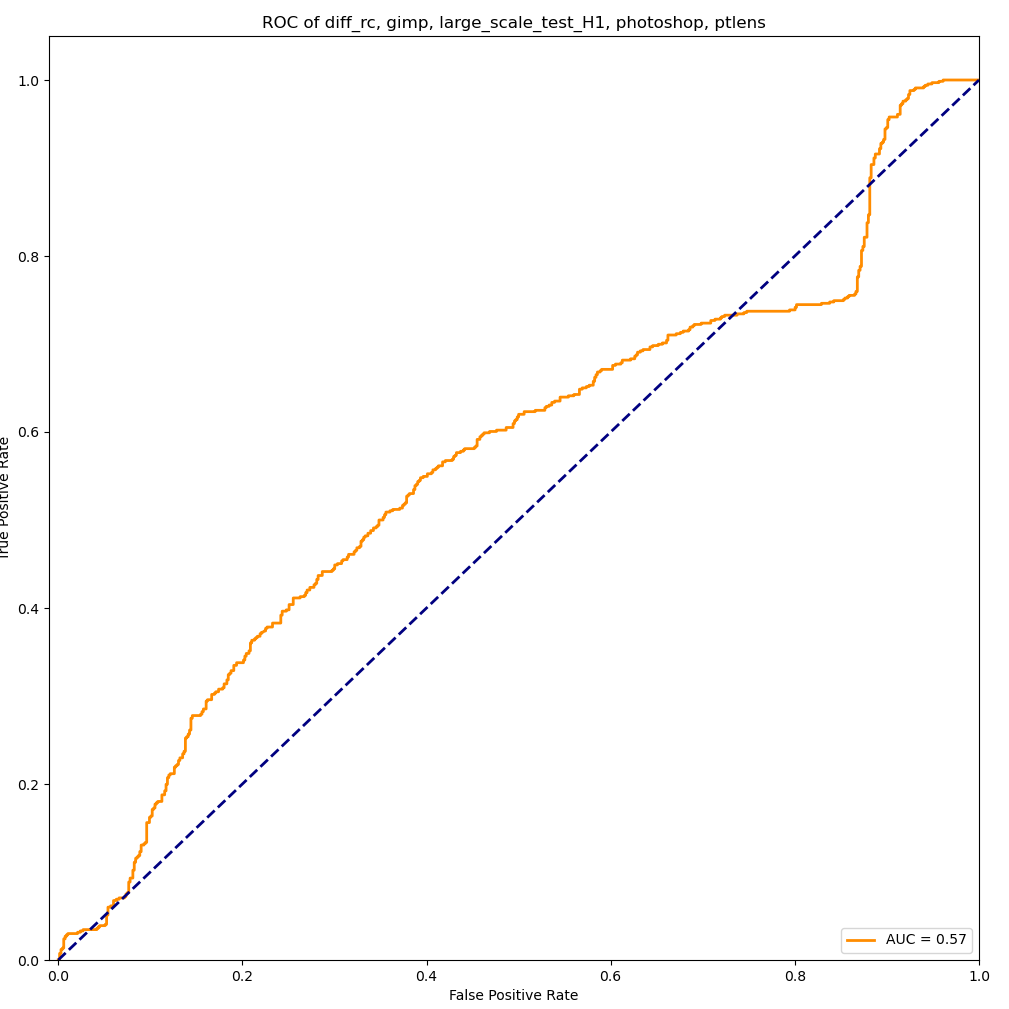
\includegraphics[width=.48\textwidth]{../drawable/results/roc-bulk__5654-all-outcamera.png}} 
        \captionsetup{justification=centering}
        \caption{ROC curves for the Dresden and Outcamera dataset.\\
        Left: $AUC = 0.91$; Right: $AUC = 0.57$}
    \end{figure}
\end{frame}

\begin{frame}{ROC curve (both datasets; $AUC = 0.77$)}
    \vspace{-1.6em}
    \begin{figure}
        \centering
        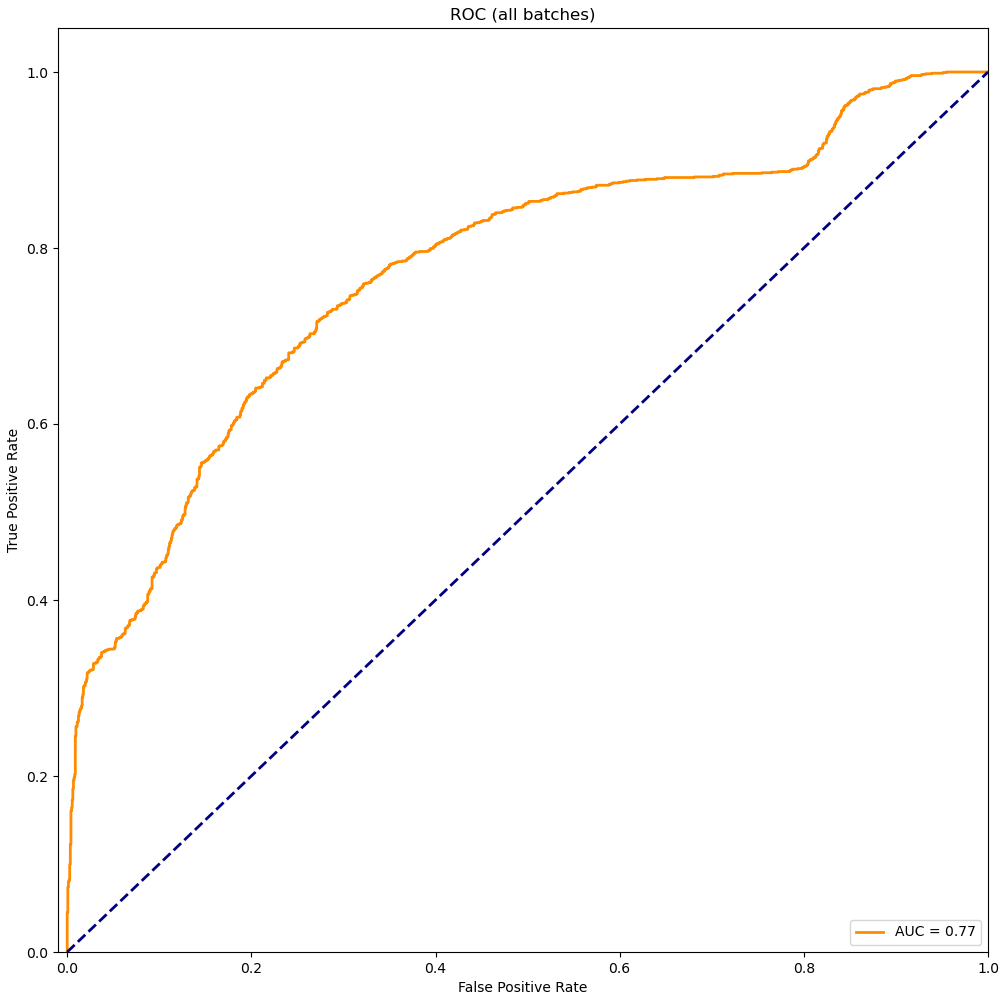
\includegraphics[height=.8\textheight]{../drawable/results/roc-bulk__7700-all-both.png}
    \end{figure}
\end{frame}

\begin{frame}{Tables - TPR/FPR Dresden}
    \vspace{-1em}
    \begin{figure}
        \centering
        \subfloat{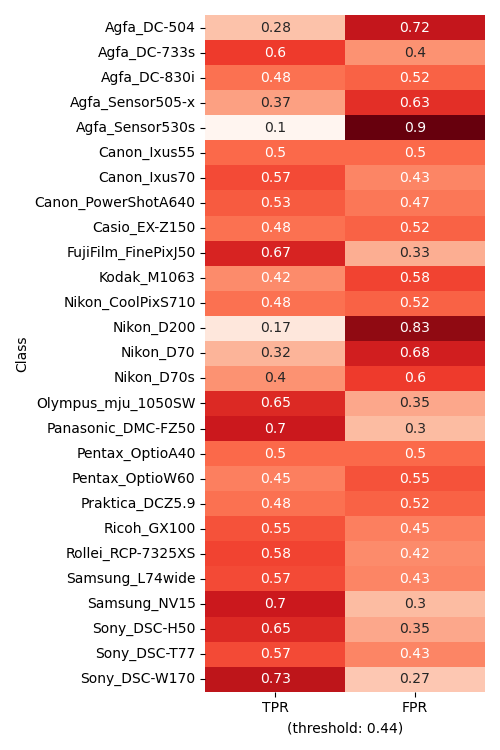
\includegraphics[width=.42\textwidth]{../drawable/results/conftable-dresden.png}}
    \end{figure}
\end{frame}


\begin{frame}{Tables - TPR/FPR Outcamera}
    \vspace{-1em}
    \begin{figure}
        \centering
        \subfloat{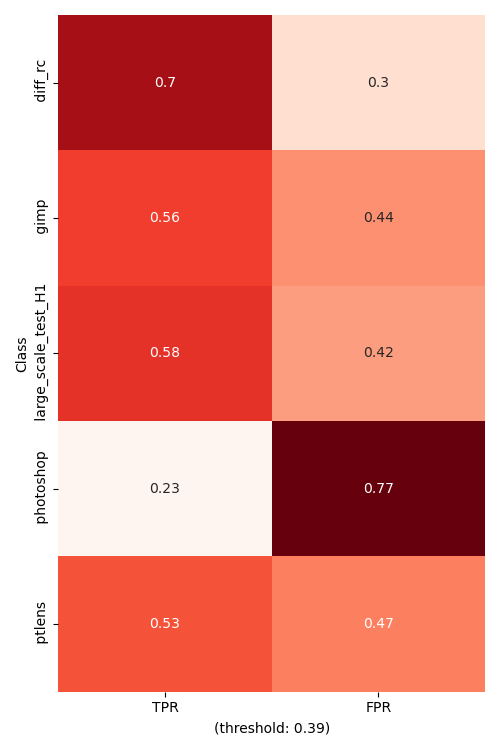
\includegraphics[width=.4\textwidth]{../drawable/results/conftable-outcamera.png}}
    \end{figure}
\end{frame}

\begin{frame}{Tables - TPR/FPR combined}
    \vspace{-1em}
    \begin{figure}
        \centering
        \subfloat{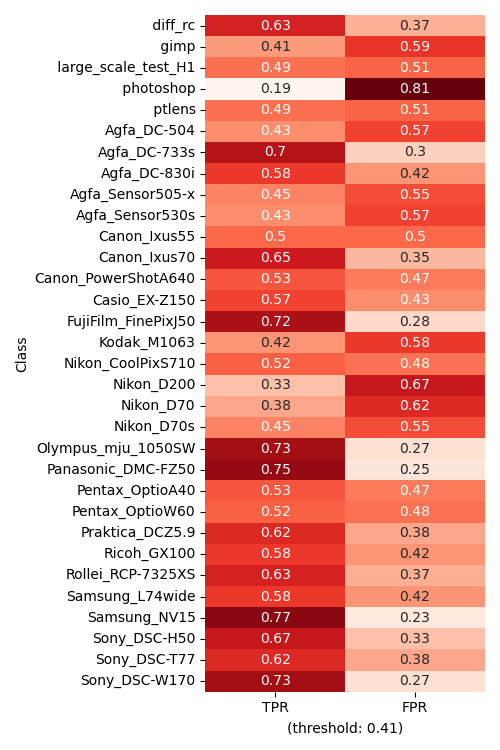
\includegraphics[width=.4\textwidth]{../drawable/results/conftable-all.png}}
    \end{figure}
\end{frame}

\begin{frame}{Setting the thresholds}

    \begin{table}[]
        \centering
        \begin{tabular}{|l|c|c|c|c|}
            \hline
            \textbf{Experiment} & \textbf{0.2 FPR} & \textbf{0.1 FPR} & \textbf{0.05 FPR} & \textbf{Optimal} \\
            \hline
            \texttt{dresden} & 0.4207 & 0.4941 & 0.5294 & 0.4411 {\footnotesize (0.1630 FPR)}\\
            \texttt{outcamera} & 0.4490 & 0.4993 & 0.5221 & 0.3864 {\footnotesize (0.4324 FPR)} \\
            \texttt{all} & 0.4364 & 0.4951 & 0.5280 & 0.4081 {\footnotesize (0.2785 FPR)} \\
            \hline
        \end{tabular}
        \captionsetup{justification=centering}
        \caption{Alternative thresholds, chosen using the \textit{set FPR} method, and the optimal one, chosen with the \textit{minimum ROC distance} method~\cite{roc-curve}}.
    \end{table}
    
\end{frame}

\section{Future work}

\begin{frame}{Multiclass classification}
    The availability of a large number of fingerprints means that Noiseprint translates decently in a multiclass classification scenario.
    
    \medskip
    
    Being trained on the Dresden database, Noiseprint performs accurately for some models and terribly for others, coherently with the paper results.
    
    \medskip
    
    A larger and more diverse dataset could allow Noiseprint to be re-trained on newer camera models.
\end{frame}

\begin{frame}{Confusion matrix - Dresden}
    \vspace{-.9em}
    \begin{figure}
        \centering
        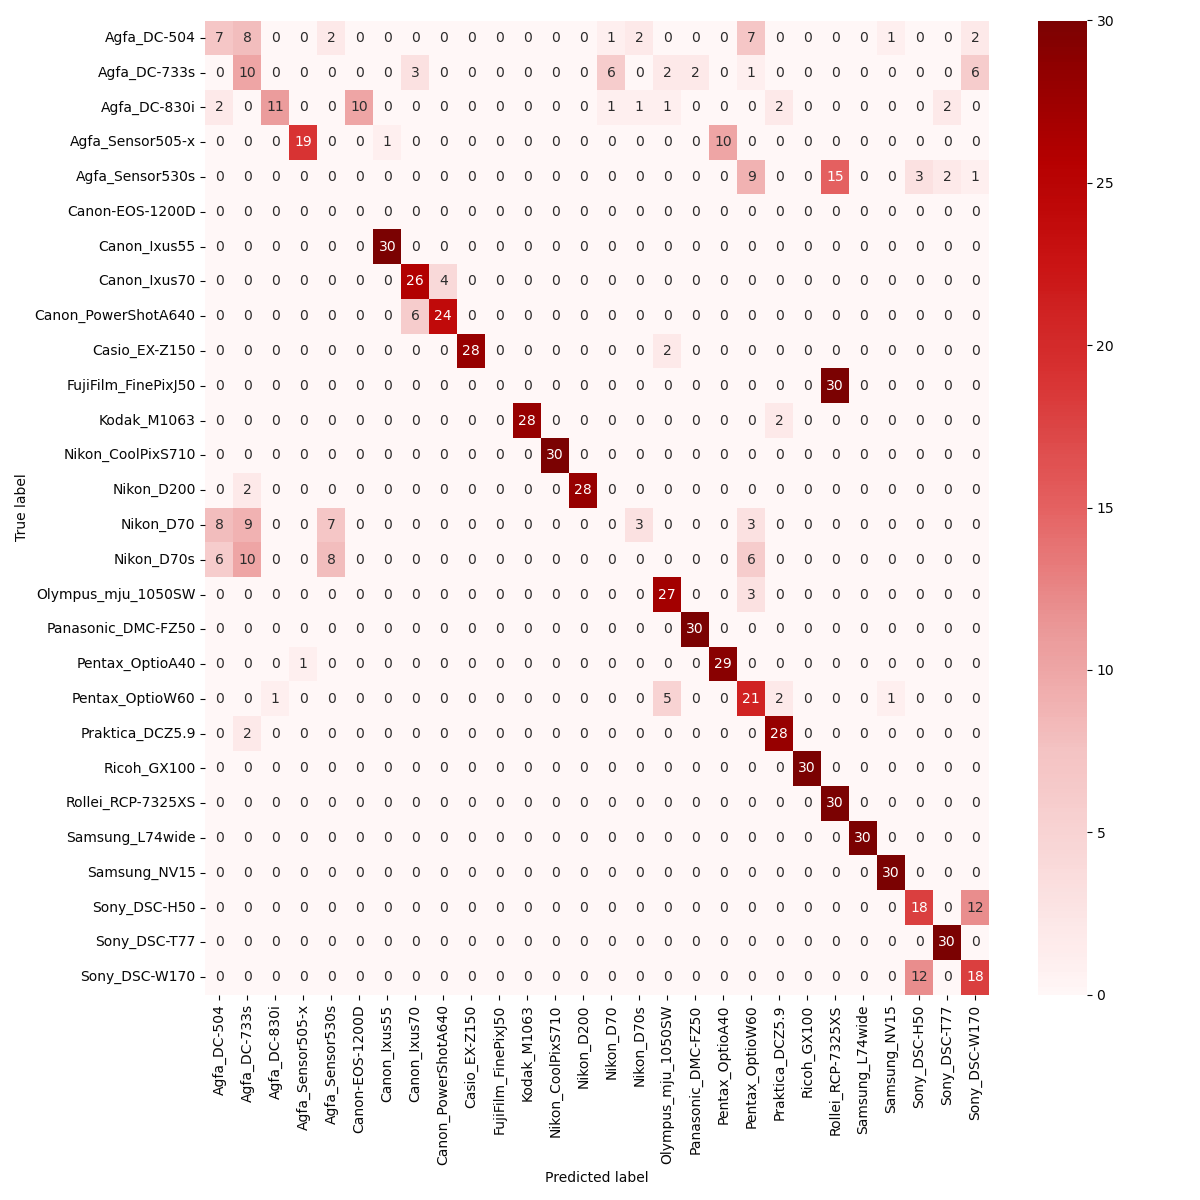
\includegraphics[height=.87\textheight]{../drawable/results/confmatrix-dresden.png}
    \end{figure}
\end{frame}

\begin{frame}{Confusion vector - Canon EOS 1200D}
    \vspace{-.9em}
    \begin{figure}
        \centering
        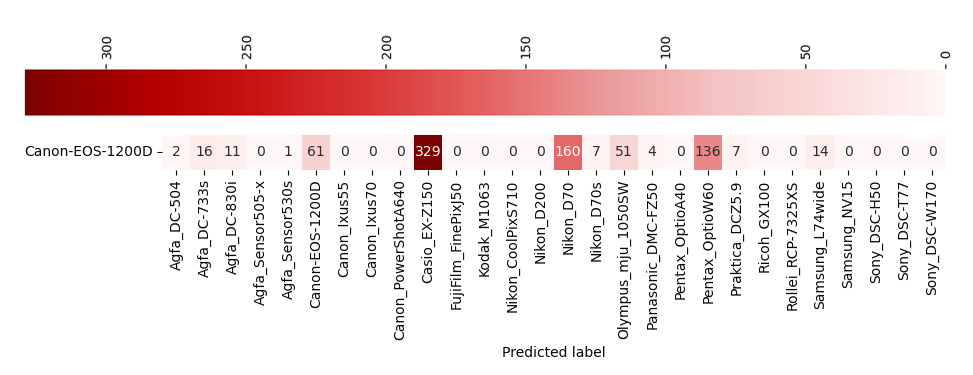
\includegraphics[width=\textwidth]{../drawable/results/confmatrix-outcamera-cropped.png}
    \end{figure}
\end{frame}

\section{References}

\begin{frame}{References}
    \bibliographystyle{IEEEtran-sorted-tt}
    \bibliography{biblio}
\end{frame}

\section{Appendix}

\begin{frame}[fragile]{Extra: code for reordering photos}

    We can sort the database with these commands.

    \begin{lstlisting}
ls | sed -r "s|^(.*)_([0-9]*)_(.*) mv \1_\2_\3 \1|g" \
   > ../move.sh
    
ls | sed -r "s/^(.*)_([0-9]*)_.*/\1/g" \
   | uniq | xargs mkdir -p
   
../move.sh
    \end{lstlisting}
    
    \medskip

    We can now get the amount of photos per folder:

    \medskip
    
    \begin{lstlisting}
for d in *; do cd $d && ls | wc -l && cd ..; done
    \end{lstlisting}

\end{frame}
\begin{frame}[fragile]{Extra: code for selecting random photos}

    To select 20 random pictures:
    
    \medskip
    
    \begin{lstlisting}
for d in *; do cd $d && ls | shuf | head -n 20 
          | xargs -I {} /bin/mv {} ../.. && cd ..; done
    \end{lstlisting}
\end{frame}

\begin{frame}{Extra: output of \texttt{verify-all-sizes.sh}}
    
    \begin{figure}
        \centering
        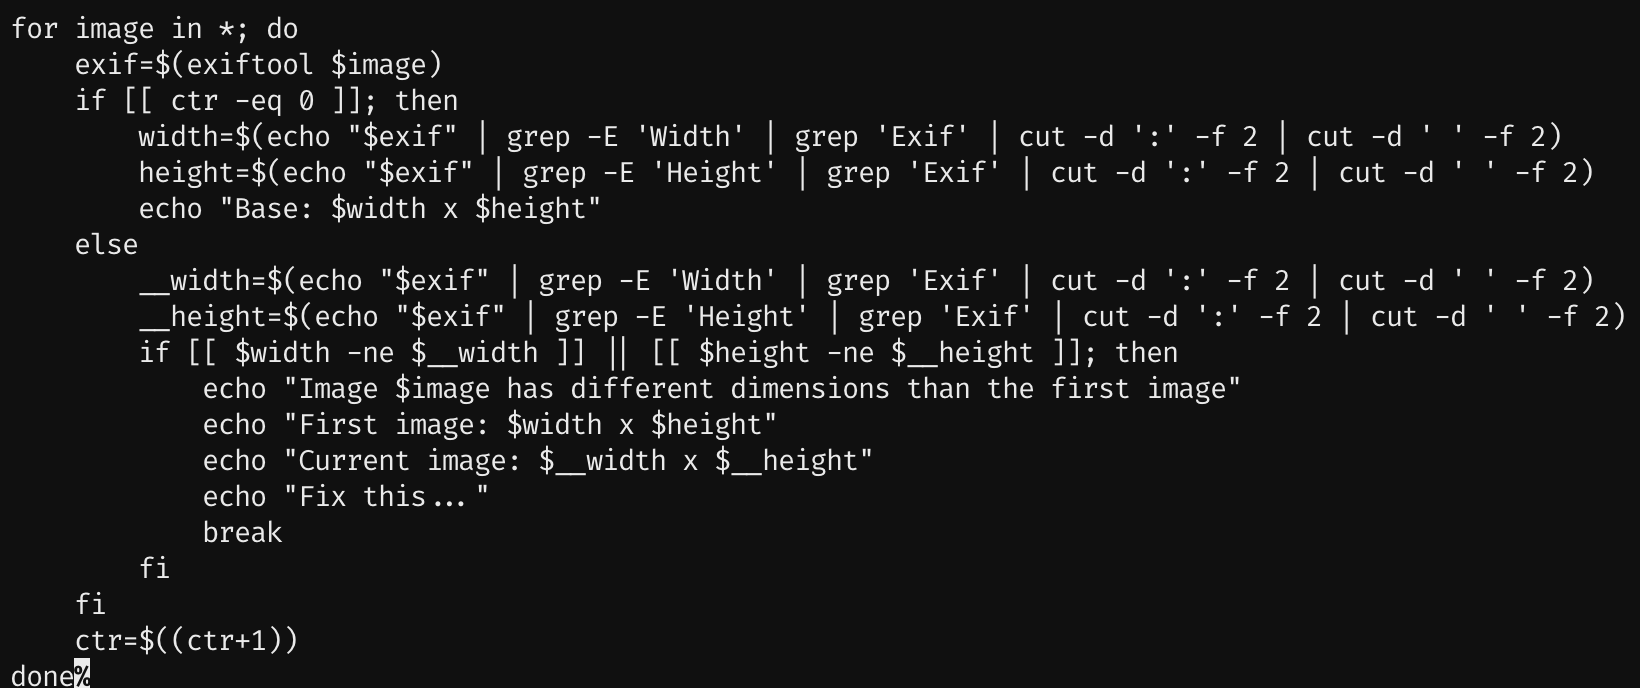
\includegraphics[width=\textwidth]{../drawable/screenshot-verifysizes.png}
    \end{figure}
    
\end{frame}

\begin{frame}{Extra: example of JSON output}
    \begin{figure}
        \centering
        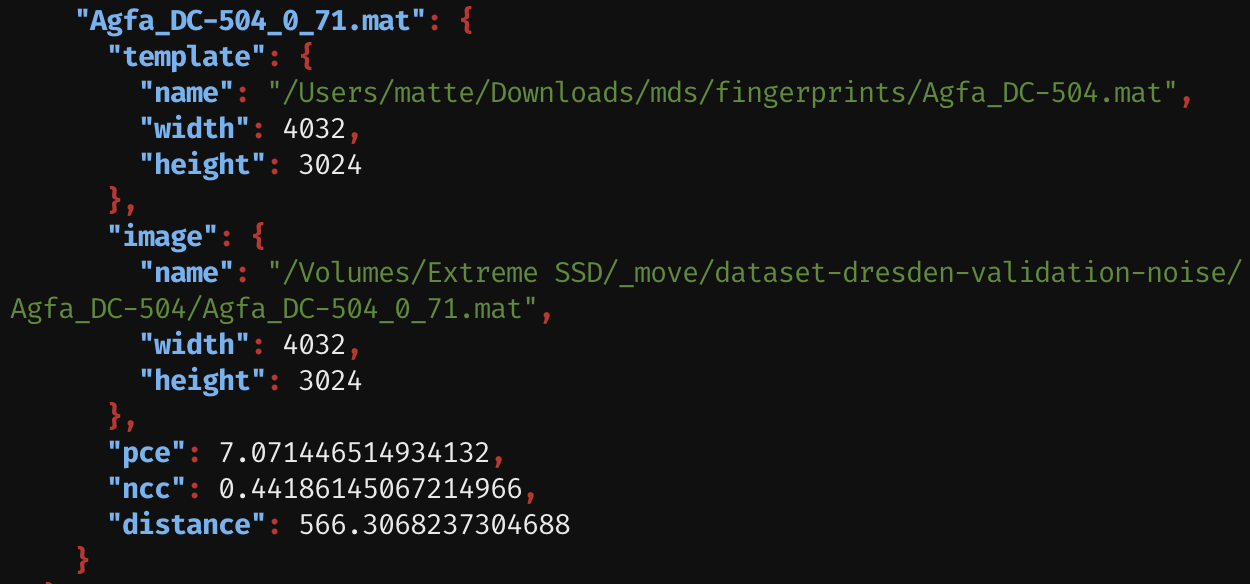
\includegraphics[width=\textwidth]{../drawable/examples/example-output.png}
    \end{figure}
\end{frame}